%%%% ijcai09.tex

\typeout{Predicting NBA Draft Position for Basketball Prospects}

% These are the instructions for authors for IJCAI-09.
% They are the same as the ones for IJCAI-07 with superficical wording
%   changes only.

\documentclass{article}
% The file ijcai09.sty is the style file for IJCAI-09 (same as ijcai07.sty).
\usepackage{ijcai09}

% Use the postscript times font!
\usepackage{times}

% Template-specific packages
\usepackage[utf8]{inputenc} % Required for inputting international characters
\usepackage[T1]{fontenc} % Output font encoding for international characters
\usepackage{mathpazo} % Use the Palatino font

\usepackage{graphicx} % Required for including images

\usepackage{booktabs} % Required for better horizontal rules in tables

\usepackage{listings} % Required for insertion of code

\usepackage{enumerate} % To modify the enumerate environment

\usepackage{dblfloatfix} % To allow pushing table and figures to bottom of page
\usepackage{caption}
\usepackage{subcaption}

\usepackage{floatrow}
% Table float box with bottom caption, box width adjusted to content
\newfloatcommand{capbtabbox}{table}[][\FBwidth]

% the following package is optional:
%\usepackage{latexsym} 

% Following comment is from ijcai97-submit.tex:
% The preparation of these files was supported by Schlumberger Palo Alto
% Research, AT\&T Bell Laboratories, and Morgan Kaufmann Publishers.
% Shirley Jowell, of Morgan Kaufmann Publishers, and Peter F.
% Patel-Schneider, of AT\&T Bell Laboratories collaborated on their
% preparation.

% These instructions can be modified and used in other conferences as long
% as credit to the authors and supporting agencies is retained, this notice
% is not changed, and further modification or reuse is not restricted.
% Neither Shirley Jowell nor Peter F. Patel-Schneider can be listed as
% contacts for providing assistance without their prior permission.

% To use for other conferences, change references to files and the
% conference appropriate and use other authors, contacts, publishers, and
% organizations.
% Also change the deadline and address for returning papers and the length and
% page charge instructions.
% Put where the files are available in the appropriate places.

\title{Predicting the Draft Slot of NBA Prospects in the Modern Era}
\author{Kevin Hillyard \& Brent George \\
CS 472, Winter 2021 \\
Department of Computer Science\\
Brigham Young University}

\begin{document}

\maketitle

\begin{abstract}
  Every year experts attempt to determine which basketball players are the most
  valuable and when those players should be picked in the NBA draft. In this
  paper, we record our efforts to accurately predict where players would be
  drafted based on their amatuer statistics using different machine learning
  models. We first describe by what means our data was gathered and what type of
  data we gathered. We then review the results we had in predicting a player’s
  draft position with our different models, namely KNN, decision tree,
  multi-layer perceptron, and linear regression. We then review our findings,
  especially from linear regression, in summarizing which statistics were
  important, and which were not as important. Lastly our ideas for future work
  and improvements to our research are made known.
\end{abstract}

\section{Introduction}

NBA scouts are always looking for NBA potential players. When determining how
good a player is, they are almost always compared to past players. Many analysts
have a general idea if a player will be a lottery pick, but the late first round
and second round predictions can vary widely.

In our research we attempted to use machine learning models to predict where a
player would be drafted. These models use the past 11 years of NBA draft
results, along with the players’ associated statistics, to determine where the
player should be drafted, if they are to be drafted at all.

The models we used were Decision Tree, KNN-Regressor, Linear Regression, and
Multi-Layer Perceptron (MLP). For each of these models we trained them on three
different datasets with a variety of hyperparameters. The three datasets we used
were a variation of our entire dataset. The first dataset only included players
that were actually drafted, the second included all players, both drafted
and undrafted, while the third included both drafted and undrafted players but
without features that were deemed less important.

There was some difficulty in predicting a player’s draft position as it is a
human perception of that player’s capability and is often swayed by what each
NBA teams’ current needs are. A possession-based point guard may have the
background of a \#15 pick, but if they meet a need of a team picking \#5, they
may be drafted at that slot. Additionally, human general managers can make
baffling decisions. In 2012, Anthony Bennett was regarded as a late first round
pick by the majority of the NBA, perhaps a fringe lottery pick. However, the
Cleveland Cavaliers, who owned the \#1 pick in the draft, selected him at that
slot. He proved to be one of the biggest busts in NBA history, failing to even
make an NBA roster only three years after being the first draft pick. Any
machine learning model would have difficulty predicting his true draft slot.

The size of our dataset is inherently limited by the size of the NBA draft. We
were also limited to a certain number of drafts as the era of basketball has
changed, encouraging more long range field goals compared to years prior. This
drastically affects the typical stats for players making comparisons between
newer and older players less viable.

Despite those difficulties we were able to predict a player’s draft position to
within 10 picks. In a future study if we were to account for the aforementioned
issues the accuracy of our results could be increased.

\section{Methods}

\subsection{Data Source}

There are various online providers of basketball statistics. Official sources
include NBA.com and the official site of NCAA basketball. However, official
sources often do not include more than the most basic statistics.

Several sites exist that provide extensive college statistics. Many of these
have a paywall (kenpom.com) or do not include statistics for international
prospects. Other sites request not to be scraped by bots.

After further exploration, we found realgm.com, a site that consented to limited
scraping that also included historical data for past statistics, data on
international prospects, and a wide array of advanced statistics. We wrote a web
scraper in Python to traverse the element tree of the web page and lift each of
the players selected in the past 11 NBA drafts and every available statistics
associated with those 660 players. This formed our initial dataset, which was
stored in a CSV file. We also pulled the records of nearly 736 prospects that
went undrafted during that same time period. 

\subsection{Featurization of Data}

Due to the nature of basketball statistics, the data scraped from the website
was already largely in the form we needed. We wrote a Python script to perform a
few sanitizing steps and convert the CSV file to an ARFF file.

The main sanitization we needed to perform was the consolidation of various
leagues that prospects played in. Prospects played in over 35 leagues and
countries. While there was consistency for prospects that played in the NCAA in
the United States, there was extreme fragmentation among the teams and leagues
that international prospects played for. In order to help the model, we grouped
all international teams under one label, leaving us with three total league
labels: NCAA, G-League, and International.

While drafted players were labeled according to their draft selection, the
undrafted players that we pulled were unlabeled. We didn’t want to use a
clustering algorithm to label these instances - a clustering algorithm would
attempt to label these players with a pick number from 1 to 60, whereas we
wanted to be able to predict if a player went undrafted. We decided to label any
undrafted player as being picked 61st, with the plan of interpreting our future
model’s output under this assumption. This led to over half of our dataset
consisting of players “selecting 61st in the draft”. This would prove to have
some positive effects, such as giving the model many examples of poor prospects
on the higher end of the draft. It would also have negative effects, such as
leading the models to be biased towards higher pick numbers when it was unsure. 

Most of our chosen features were already real values, and directly translated to
our final dataset. We had two nominal features, position and league. We decided
to do a binary encoding for each of these two features, trusting that higher
complexity models would be able to interpret this and differentiate the value of
various statistics per position. For example, we would anticipate that the model
would value rebounds and blocks for a center more than for a point guard. This
may not be a necessary distinction in the end, but we wanted to give our models
the chance to pick up on it.

\subsection{Models}

We used a variety of models in this project, to be described in further detail
in results sections. All implementations came from scikit learn v1.0.1.

\section{Initial Results}

Initially, we trained Decision Tree, Multi-Layer Perceptron, KNN-Neighbor, and
Linear Regression models. Each of these had a grid of hyperparameters that was
exhaustively searched to find the best results, as recorded in Tables
\ref{tab:dt_grid}, \ref{tab:mlp_grid}, and \ref{tab:knn_grid}.

\begin{table*}
	\begin{center}
		\begin{tabular}{||c c c c c c||} 
		\hline\hline
		Hyperparameter & Opt. 1 & Opt. 2 & Opt. 3 & Opt. 4 & Opt. 5 \\ 
		\hline\hline
		Criterion & Squared Error & Friedman MSE & Absolute Error & Poisson & \\ \hline 
		Splitter & Best & & & &  \\ \hline
		Max Depth & 8 & 16 & 24 & 32 & 48 \\ \hline
		Min Samples for Split & 2 & 4 & 6 & &  \\ \hline
		Min Samples per Leaf & 1 & 2 & 4 & &  \\ \hline
		Min Weight Fraction per Leaf & 0.0 & 0.001 & 0.01 & &  \\ \hline
		Min Impurity Decimal & 0.0 & 0.001 & 0.01 & &  \\
		\hline\hline
		\end{tabular}
	\end{center}
	\caption{Decision Tree Hyperparameter Grid}
	\label{tab:dt_grid}
\end{table*}

\begin{table*}
	\begin{center}
		\begin{tabular}{||c c c c c c||} 
		\hline\hline
		Hyperparameter & Opt. 1 & Opt. 2 & Opt. 3 & Opt. 4 & Opt. 5 \\ 
		\hline\hline
		Hidden Nodes & (64) & (128) & (64, 64) & (64, 32, 64) & (128, 128) \\ \hline
		Learning Rates & 0.01 & 0.1 & 0.2 & 0.5 & 1.0 \\ \hline
		Momentum & 0.0 & 0.3 & 0.5 & 0.8 & 1.0 \\ \hline
		Regularization & 0.0001 & 0.0005 & 0.001 & & \\ 
		\hline\hline
		\end{tabular}
	\end{center}
	\caption{Multi-Layer Perceptron Hyperparameter Grid}
	\label{tab:mlp_grid}
\end{table*}

\begin{table*}
	\begin{center}
		\begin{tabular}{||c c c c c||} 
		\hline\hline
		Hyperparameter & Opt. 1 & Opt. 2 & Opt. 3 & Opt. 4 \\ 
		\hline\hline
		K & 1 & 3 & 5 & 7 \\ \hline
		K continued & 9 & 11 & 13 & 15 \\ \hline
		Distance Metrics & Euclidean & Manhattan & Chebyshev & Minkowski \\ \hline
		\hline\hline
		\end{tabular}
	\end{center}
	\caption{K-Nearest Neighbors Hyperparameter Grid}
	\label{tab:knn_grid}
\end{table*}

\subsection{Without Undrafted Players}

We first trained our models on the dataset excluding all undrafted players. The
Mean Absolute Error (MAE) was fairly high, with an average of about 15 across
all hyperparameter combinations, and with minimums of about 12 picks off for the
best model and hyperparameter combinations. An issue we found with this subset
was that there were not enough bad players for the models to learn form. 

The baseline MAE for this first dataset is based off of guessing the average
pick for each prospect. The average draft slot was 30.5, and the baseline MAE
using this average was 14.976.

\subsection{Decision Tree}

After training the decision tree model on this subset it achieved a minimum MAE
of 13.689. The hyperparameters with which we achieved the best score used
poisson as the criterion, a max depth of 8 layers, minimum samples set to 6 and
4 for split and leaf respectively, and both the minimum weight fraction leaf and
minimum impurity decrease set to 0.01.

\subsection{KNN-Regressor}

When training our KNN-Regressor on the subset excluding undrafted players it
achieved a minimum MAE of 13.129. We achieved the best MAE when setting k to 9
and using a manhattan distance metric.

\subsection{Linear Regression}

The MAE our Linear Regression model achieved was a value of 11.265. No special
hyperparameters were used for this model.

\subsection{MLP}

The last model which we trained on this subset of data was our MLP. It achieved
a MAE of 11.490. The combination of hyperparameters that achieved the
best MAE had hidden nodes set to (64, 64), a learning rate of 0.2, a momentum of
0.5, and regularization of 0.0001.

\subsection{With Drafted and Undrafted Players}

As already mentioned, the lack of examples of bad players made the learning
difficult for the first round of models. The following models achieved a better
MAE when using both drafted and undafted players. The variety of talent allowed
the models to learn to recognize both good and bad players and was more accurate
as a result.

The average draft slot for this more comprehensive dataset was 46.756. Using
this average, the baseline MAE is 16.636.

\subsection{Decision Tree}

When training the decision tree on both drafted and undrafted players it
achieved a MAE of 9.560. This is an improvement from 13.689 MAE that was
achieved using the subset without undrafted players. This score would prove to
be our best overall score in our initial training. We used the same
hyperparameters mentioned before and the best score was achieved when using the
following settings: absolute error as the criterion, max depth set to 8 layers,
the minimum samples for splits set to 4 while the minimum samples for leaves was
set to 1, the minimum weight fraction leaf set to 0.01, and the minimum impurity
decrease set to 0.001.

\subsection{KNN-Regressor}

The KNN-Regressor when trained on both drafted and undrafted players achieved a
MAE of 11.699. This is 1.43 picks better than the previous KNN-Regressor model.
This score would be the worst score for all models trained on both drafted and
undrafted players. The score was achieved using the same hyperparameters as
before but with a k value of 3 using a euclidean distance metric.

\subsection{Linear Regression}

Our Linear Regression model had the third best initial score with a MAE of
10.091. This is an improvement from the previous Linear Regression model that
scored 11.265.

\subsection{MLP}

Lastly our MLP had the second best initial score with a MAE of 9.851. It used
the same hyperparameters as the previous MLP model, but had the following
settings: hidden nodes was set to 128, learning rate was set to 0.1, momentum
was set to 0.8, and we used a regularization value of 0.0001. Compared to the
first MLP model not trained on undrafted players, this model improved that score
by 1.588.

\subsection{Summary of Initial Results}

Figure \ref{fig:initial_results} shows a visual for the best results for our
initial models. The models trained with the undrafted players included performed
much better on average. However, there wasn't much differentiation between the
MLP, Decision Tree, and Linear Regression models with that dataset, suggesting
that none had a particular advantage for our compiled datasets.

\begin{figure}
	\begin{center}
	\makebox[\textwidth][c]{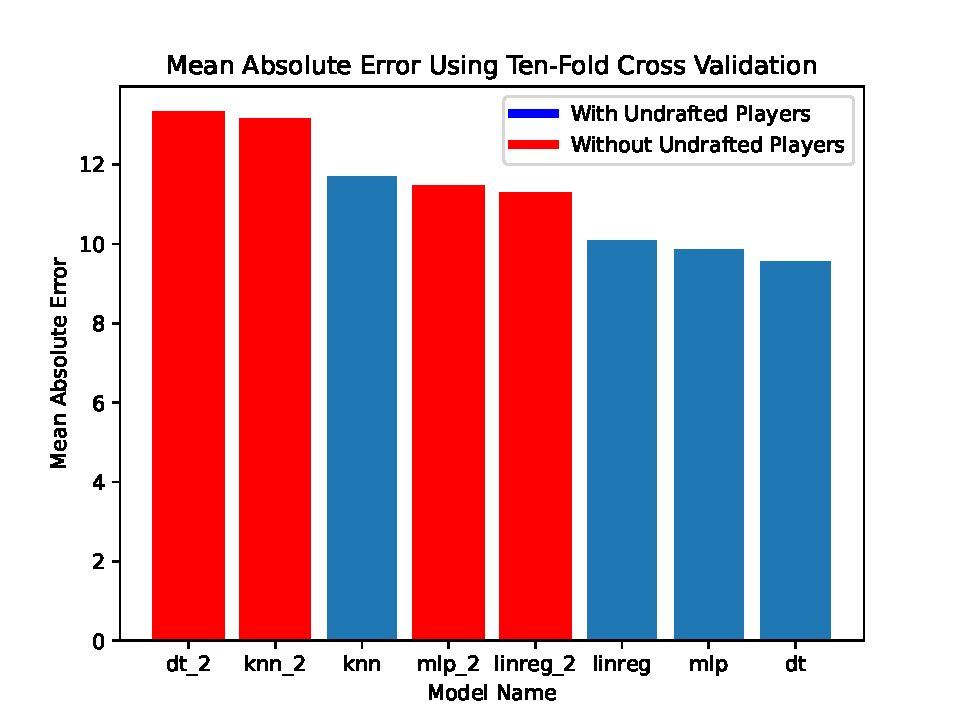
\includegraphics[width=1.1\textwidth]{error_by_model.pdf}}
    \caption{Bar Chart of Mean Absolute Error for Each Initial Model}
    \label{fig:initial_results}
	\end{center}
\end{figure}

\section{Feature and Model Improvements}

To improve our results we reviewed the most important features and least
important features as determined by the weights from our linear regression
model. The features that had the lowest weights included the following features:
Usage \%, Assist \%, Field Goals Made, Field Goals Attempted, Free Throws Made,
Free Throws Attempted, 3-pointers Made, and 3-pointers Attempted. We deemed
these features safe to remove as they had low weights and the essence of their
value was captured in a different feature. For example, Field Goals Made and
Field Goals Attempted is captured in the feature Field Goal \% which had a high
weight. In removing these somewhat redundant features we hoped to slightly
improve our predictions, especially for the KNN model. We didn't weight the
values of various features when calculating the distance between neighbors, so
if we had many redundant or useless features, they would drown out the important
features and make it difficult for the KNN model to be effective.

Because we reduced the number of features, but did not change the number of
instances, the baseline MAE remained unchanged. The average draft slot was
46.756 again, and the baseline MAE is 16.636.

\section{Final Results}

\subsection{Decision Tree}

When training a Decision Tree model on this new dataset we were able to achieve
a MAE of 9.718. This was the best score from all of the models trained on this
new dataset but was 0.158 higher than the Decision Tree trained on the unaltered
dataset with both drafted and undrafted players. This would be the second best
score from all of our results. This score was achieved using the following
hyperparameters: a maximum depth of 8 layers, a minimum sample of 2 for splits
and 1 for leaves, minimum weight fraction leaf of 0.01, and a minimum impurity
decrease of 0.01.

\subsection{KNN-Regressor}

The KNN-Regressor trained on the new dataset had the worst score of all models
trained on this dataset. It had a MAE of 11.790. This was better than the first
model trained on the data without undrafted players, but worse than the model
trained on all players. This score was achieved using a k value of 2 and using a
euclidean distance metric.

\subsection{Linear Regression}

Training the Linear Regression model on this new dataset resulted in a MAE of
9.987. This was the second worst of all models trained on this dataset but was
better than the other two Linear Regression models trained on the other
datasets.

\subsection{MLP}

Lastly our MLP trained on this new dataset resulted in a MAE of 9.858. This was
only 0.007 worse than the model trained on the unaltered dataset with all
players. This was the second best score of all models trained on the new dataset
and the fourth best overall. The score was achieved by using the following
hyperparameters: the hidden nodes were set to (32,32), the learning rate was
0.1, momentum was set to 0.8, and we used a regularization value of 0.001.

\subsection{Improvement Results}

\begin{figure}
	\begin{center}
	\makebox[\textwidth][c]{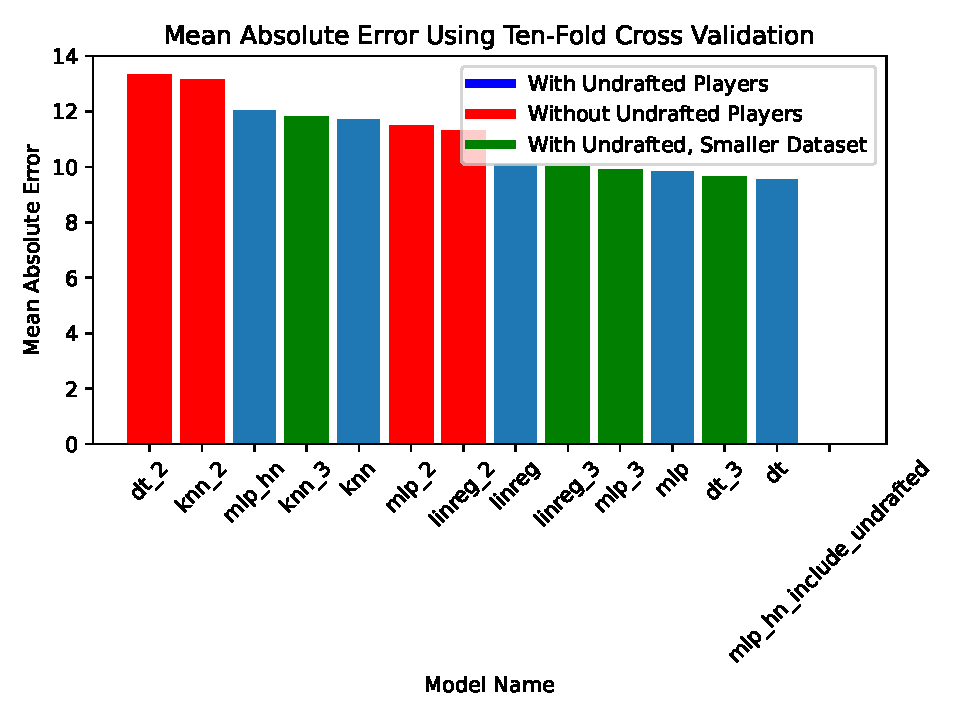
\includegraphics[width=1.1\textwidth]{error_by_model_2.pdf}}
    \caption{Bar Chart of Mean Absolute Error Including Smaller Dataset Results}
    \label{fig:improved_results}
	\end{center}
\end{figure}

The changes we made with our improvements initially surprised us as the MAE for
each model trained on the adjusted dataset was almost identical to, if not
slightly higher than, the MAE scores for the models trained on the unaltered
dataset with both drafted and undrafted players. Reviewing these results they do
match up with the behavior of the models we chose. All of our models, aside from
the KNN-Regressor, are capable of learning to ignore unnecessary features. By
removing features the linear regressor deemed less useful we most likely only
reduced the training time for our models. Concerning our KNN-Regressor the
consistently high MAE was likely due to not having enough data to effectively
make predictions from neighboring instances. This will be discussed further in
the Final Results section.

\section{Discussion and Conclusion}

Our results were largely promising, especially considering the speculative
nature of the late first round and second round of the NBA draft. Our models'
best efforts could predict a player's draft slot within about 9 picks. This is
valuable in and of itself, as many NBA prospects will hire outside counsel to
discover where they might fall in the draft. They use the counsel's predictions
to determine whether to continue to develop their game for another year, or
whether to declare for the current year's draft. Having our free ML model
available to give a first or second opinion may be of value.

Our model performed slightly better than the baseline MAE for the dataset that
only included drafted players. The baseline MAE was about 15, and our best
models had Mean Absolute Errors ranging from 11 to 13. For the datasets that
included undrafted players as well, the models outpaced the baseline MAE by a
few more points - the baseline MAE was almost 17, and our best models had Mean
Absolute Errors ranging from 9 to 11.

Unfortunately, the model does not perform better than current human standards.
In this sense, this problem is not "solved" by our approach. Future work needs
to be done to improve the results. Most expert draft analysts have a MAE of 4-5
picks every NBA draft. A model that could match or improve on this benchmark may
be possible with the improvements discussed in the next section.

\section{Future Work}

Changes we would make to our research to improve the results of our predictions
include further research about the data, how the error of our models was
determined, and additional features.

\subsection{Further Draft Research}

As previously mentioned in this report there were some contributing factors to a
player’s draft stock that we did not take into account when gathering our data.
When gathering our data on when a player was drafted it would be worthwhile to
research the team’s needs that drafted that player. Knowing this would allow us
to determine if the player was drafted at that position for their skills as a
player or more for their fit with that team. We could create a feature that
encodes how many picks higher or lower a certain prospect was drafted based on
the needs of the teams drafting in that prospect's range.

Additionally, we could do player comparisons with existing NBA players. This is
a common draft tactic used by general managers, and it might be helpful for the
models as well. This would involve gathering player profiles of successful and
unsuccessful NBA players, and using their similarity to NBA prospects to
determine if that prospect might be valued in the modern NBA.

Finally, we could improve the size of our dataset by including more drafts. This
is initially unhelpful because the shifting nature of the NBA leads to certain
players being very valuable 40 years ago and insignificant today, and vice
versa. We would have to do era adjustments on any datasets that included older
generations and thoroughly test the effectiveness of this approach.

\subsection{Error Scoring}

There was an issue with the error scoring with our models as we were using the
scikit models with their own error scoring function. Because undrafted players
don’t have a draft position associated with them we imputed their labels so that
all undrafted players were drafted 61st. 

The issue appears when our models predict a draft position greater than 61. Our
data has a max of 61 while our models are able to predict draft positions higher
than this. The error scoring for the models considers this difference as an
error, when in reality if the player has a draft position of 61 any placement
greater than or equal to 61 should be considered correct. A custom error scoring
module that plugged in to skicit learns models could dramatically improve our
results.

\subsection{Additional Features/Sources}

As a final change to our research we would gather data from one or more
additional sites in order to gather all advanced statistics possible. The site
we pulled our data from had a large number of advanced statistics but not all of
them.


\end{document}

